\section{Descripcion y Solucion del Problema}
%\lipsum[2-3] me sirve
Escribir un programa web que utilice CGI, HTML, CSS, que haga consultas sobre el archivo de universidades licenciadas.  
El archivo debe ser procesado con una expresión regular para extraer todos sus campos, al estilo del ejemplo unificado.
La consulta debe ser una respuesta a un formulario html.  Se debe de trabajar con GIT.\\

\textbf{Archivo} \\
\url{https://www.datosabiertos.gob.pe/sites/default/files/Programas de Universidades.csv}

\begin{itemize}
    \item Nombre Universidad.
    \item Periodo Licenciamiento.
    \item Departamento Local.
    \item Denominación Programa.
\end{itemize}

Para resolver este ejercicio, si bien voy a utilizar las herramientas mensionadas en el enunciado, a parte de ello utlizare
XAMPP un servidor local que cumple una funcion similar al Virtual Box. En las siguientes secciones mostrare el codigo fuente. 
\clearpage

\subsection{Codigo Fuente : Consulta.html}
%\lipsum[4]
A continuación, mostrare el codigo de la pagina principal del trabajo: \\
\begin{figure}[h!]
    \centering
    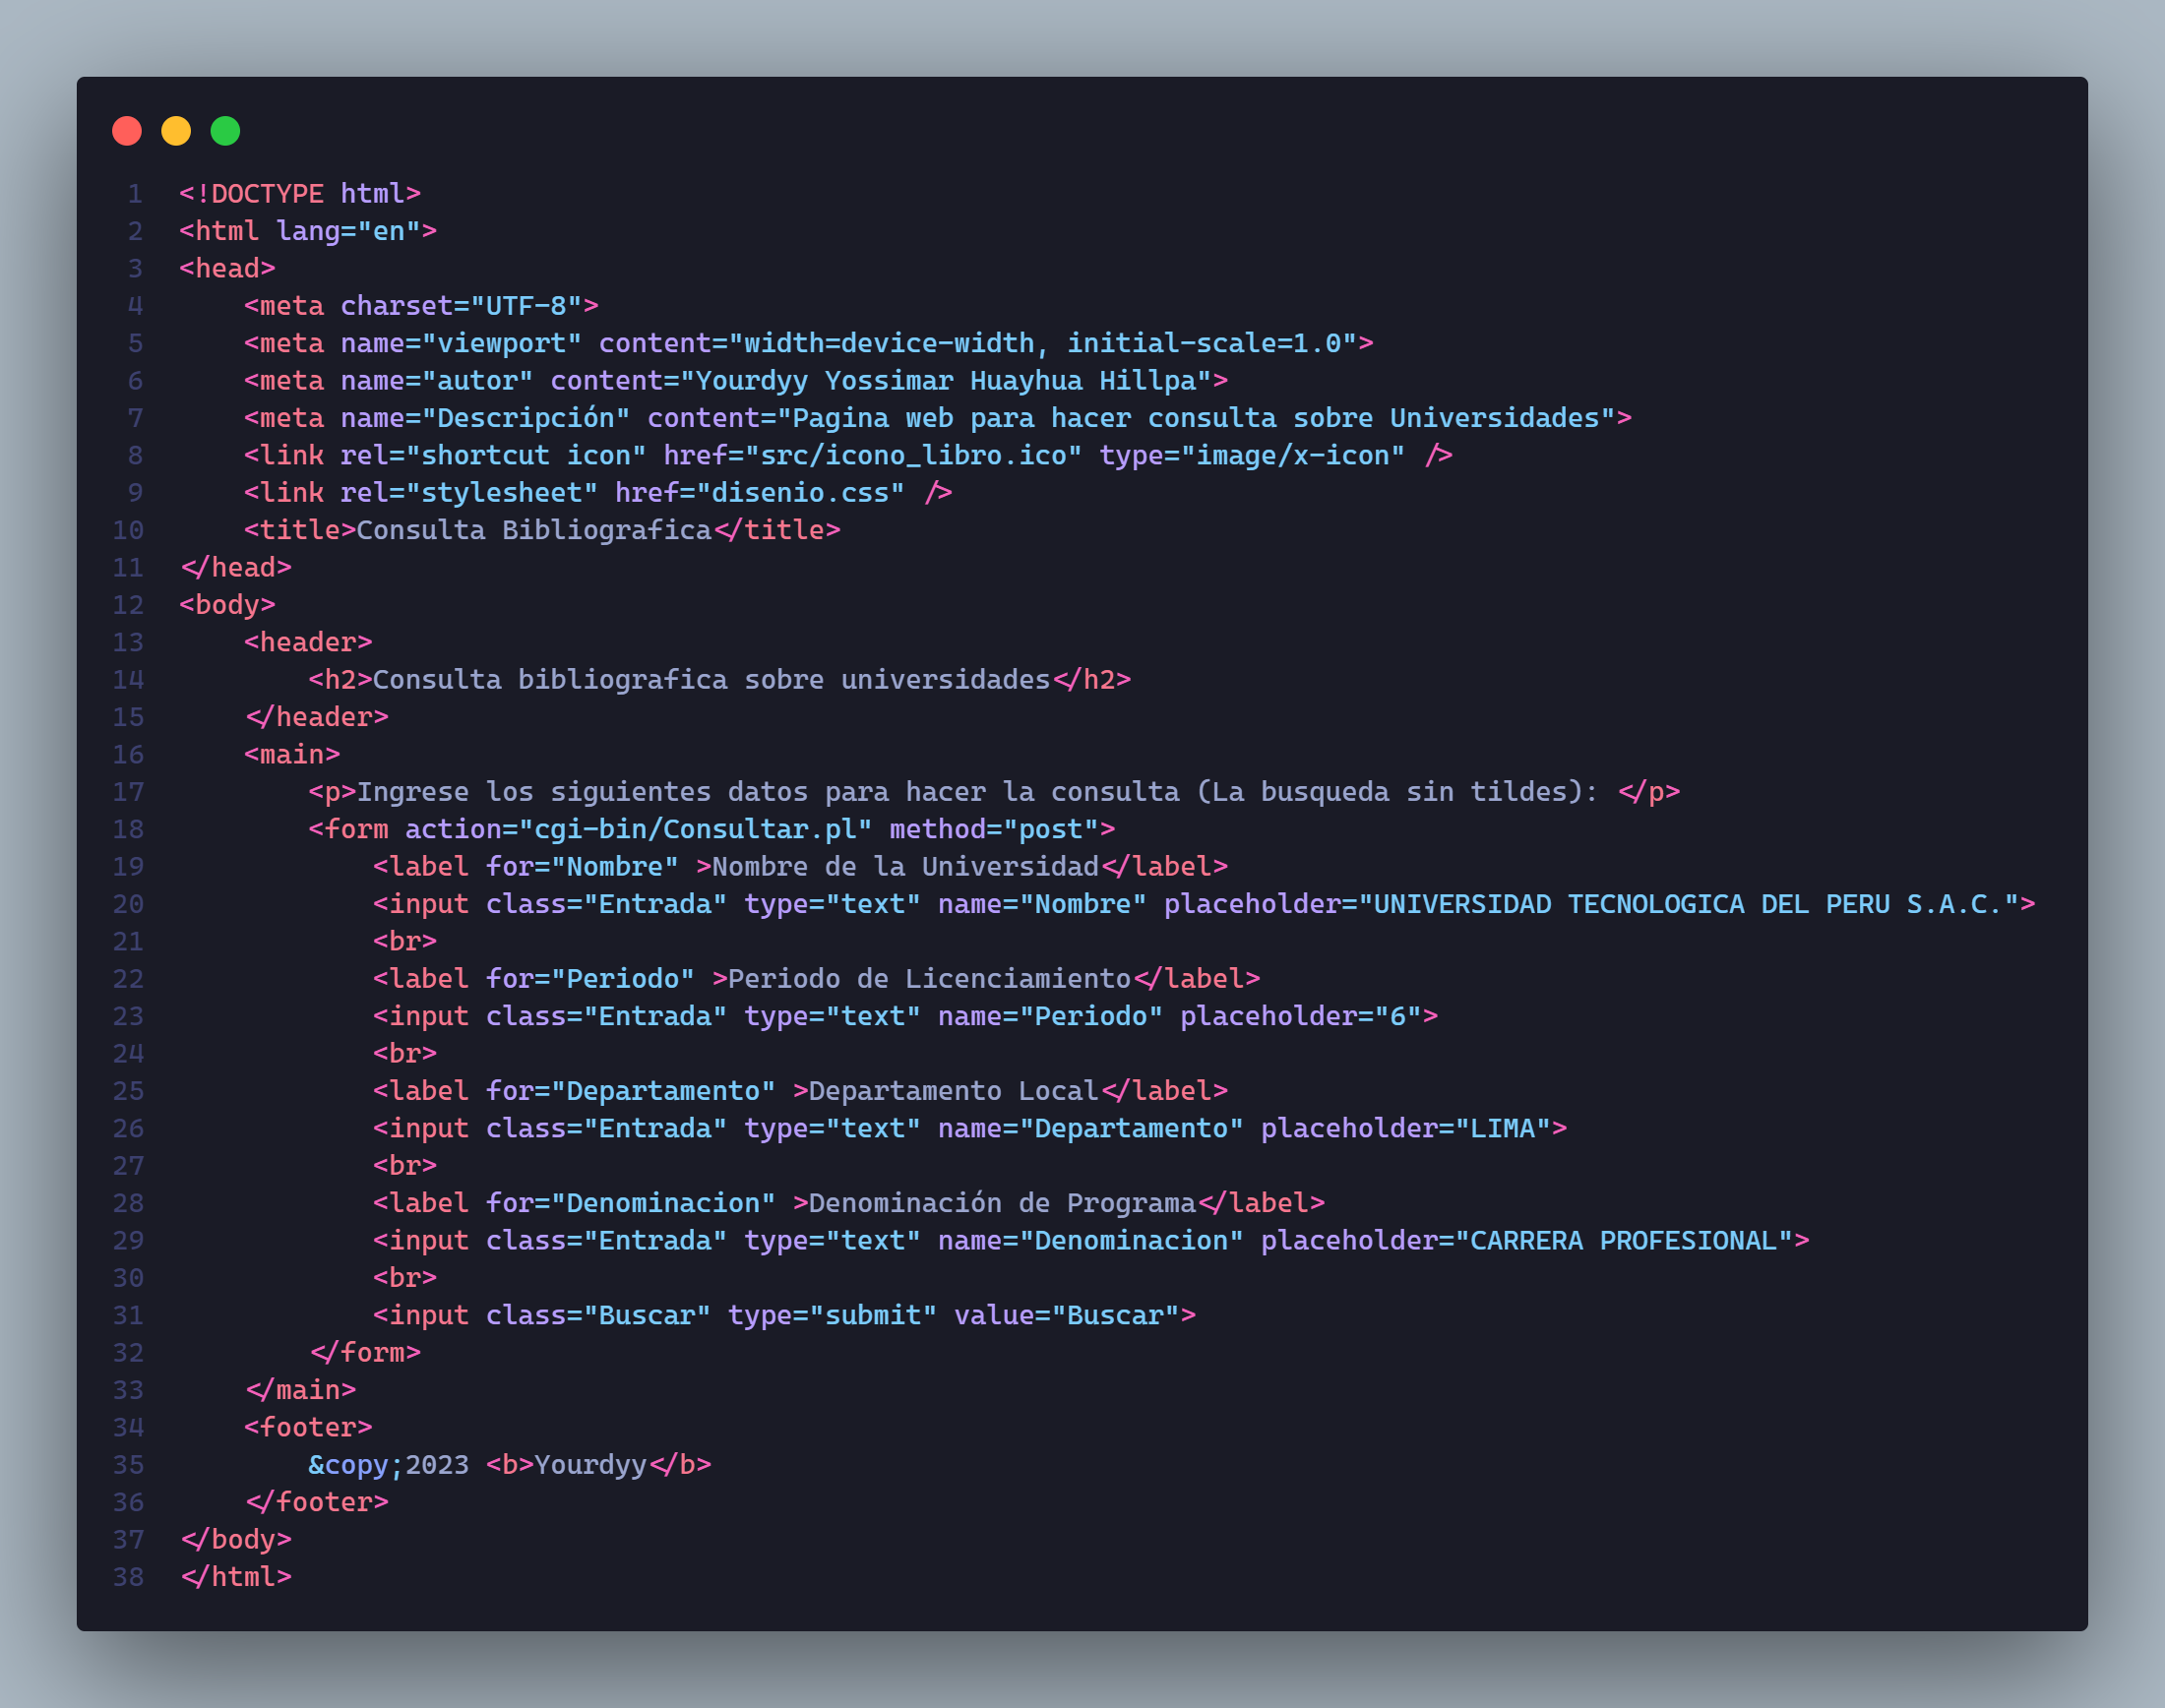
\includegraphics[width=1.0\textwidth,keepaspectratio]{img/Consulta_html.png}
    %\includesvg{img/automata.svg}
    %\label{img:mot2}
    %\caption{Product backlog.}
\end{figure}\\

\subsection{Codigo Fuente : disenio.css}
%\lipsum[5]
Ahora el codigo del diseño de las paginas web: 
\begin{figure}[h!]
    \centering
    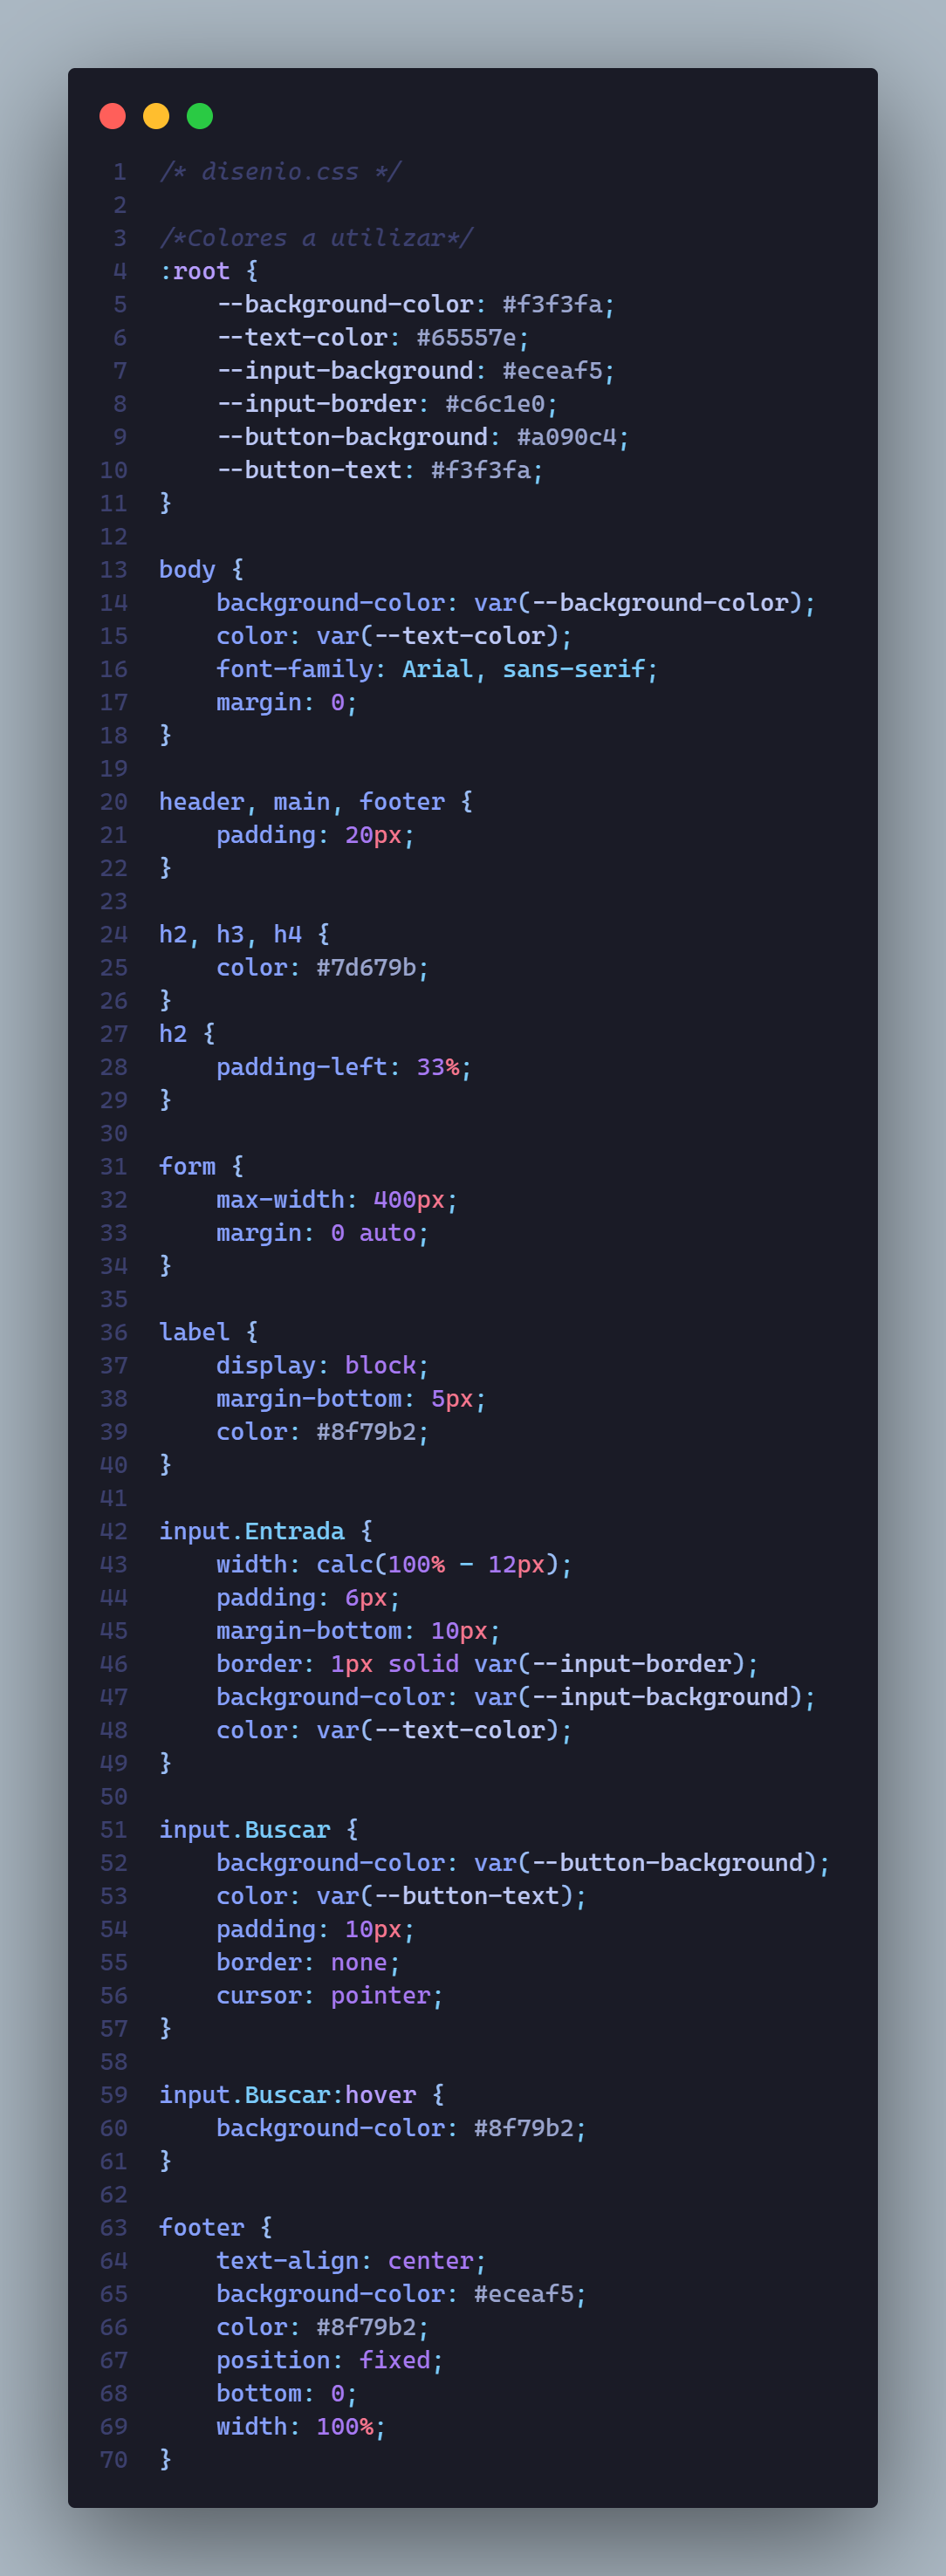
\includegraphics[width=0.5\textwidth,keepaspectratio]{img/disenio_css.png}
    %\includesvg{img/automata.svg}
    %\label{img:mot2}
    %\caption{Product backlog.}
\end{figure}
\clearpage

\subsection{Codigo Fuente : Consultar.pl}

Por ultimo el codigo del programa que maneja el archivo .csv:
\begin{figure}[h!]
    \centering
    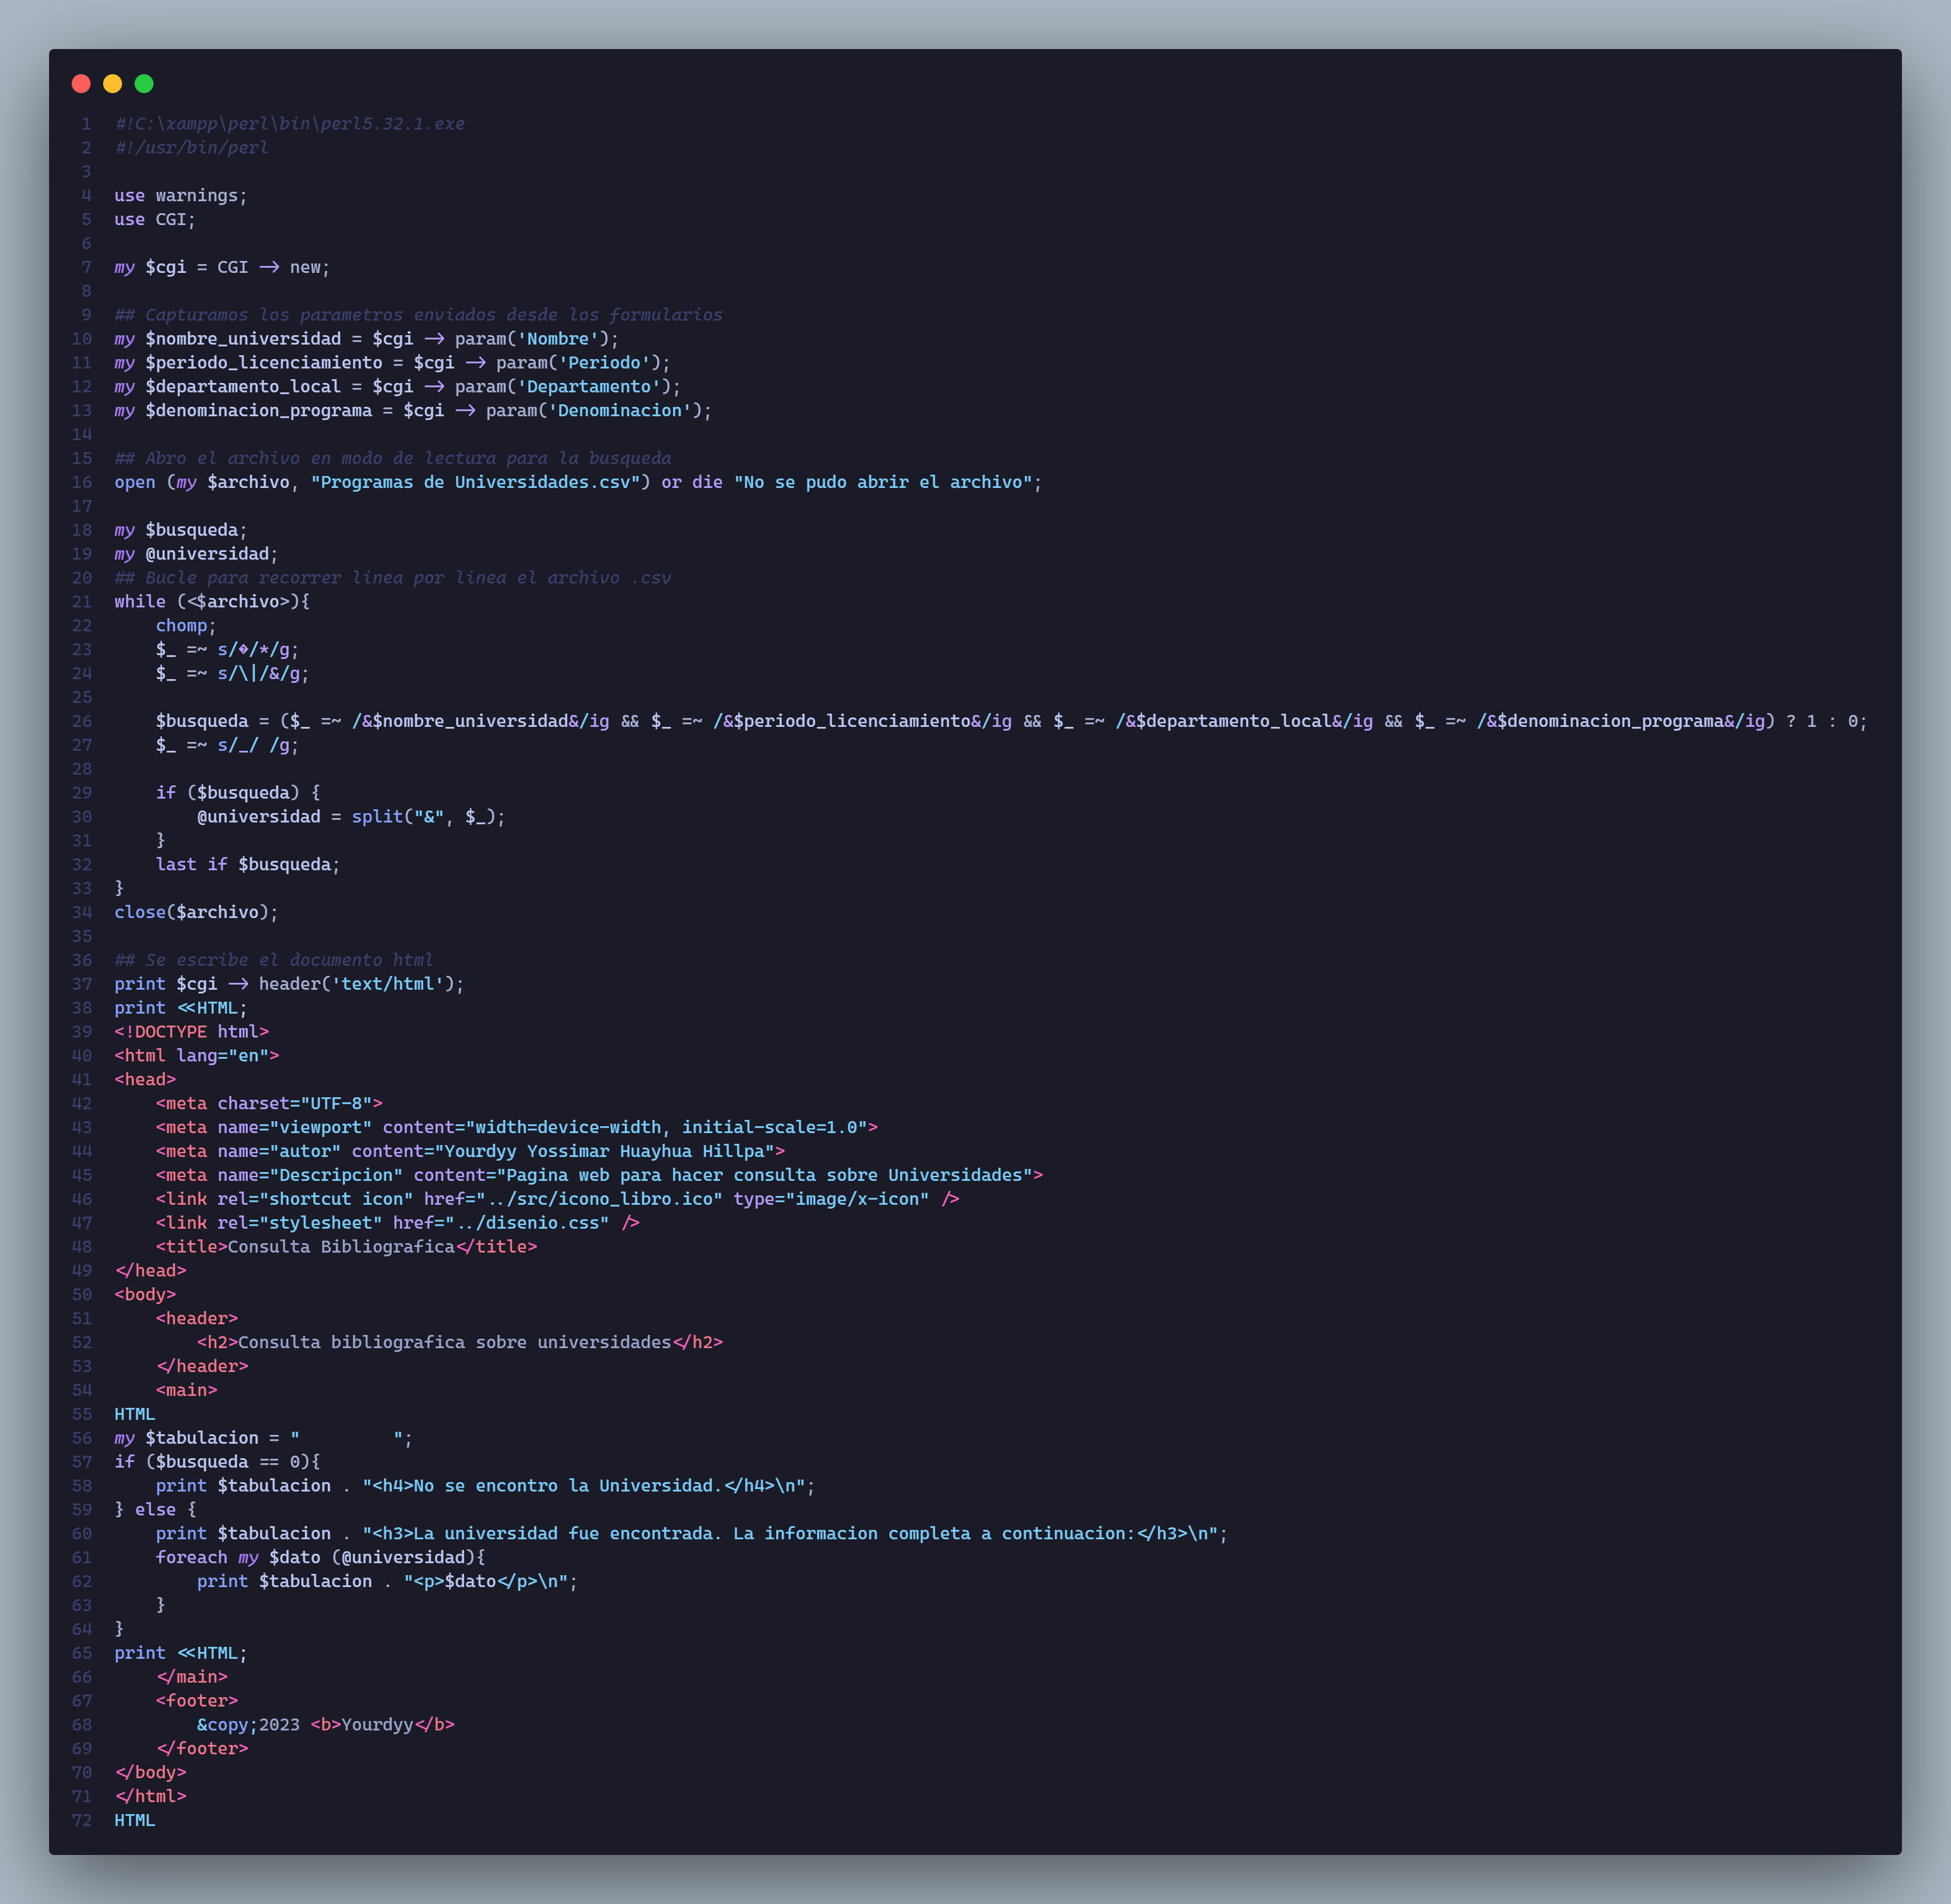
\includegraphics[width=1.2\textwidth,keepaspectratio]{img/Consultar_pl.png}
    %\includesvg{img/automata.svg}
    %\label{img:mot2}
    %\caption{Product backlog.}
\end{figure}
\clearpage

\subsection{Estructura del Laboratorio y Repositorio:}

La estructura del laboratorio es de la siguiente manera:
\begin{figure}[h!]
    \centering
    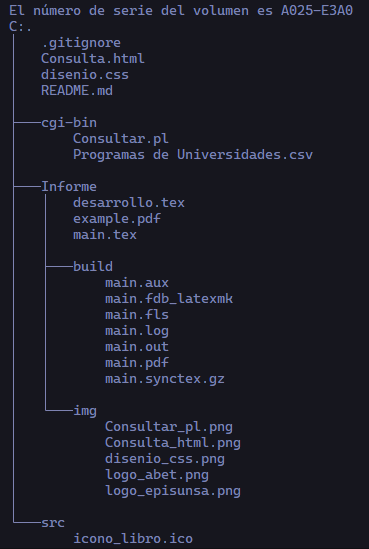
\includegraphics[width=0.6\textwidth,keepaspectratio]{img/Estructura.png}
    %\includesvg{img/automata.svg}
    %\label{img:mot2}
    %\caption{Product backlog.}
\end{figure}
\\
Repositorio GitHub:
\url{https://github.com/yhuayhuahi/Lab_09.git}

\subsection{Prueba del programa}
Capturas de pantalla, de como se muestra en el navegador:
\begin{figure}[h!]
    \centering
    
\includegraphics[width=0.8\textwidth,keepaspectratio]{img/Prueba1.png}
    %\includesvg{img/automata.svg}
    %\label{img:mot2}
    %\caption{Product backlog.}
\end{figure}
\begin{figure}[h!]
    \centering
    
\includegraphics[width=0.8\textwidth,keepaspectratio]{img/Prueba2.png}
    %\includesvg{img/automata.svg}
    %\label{img:mot2}
    %\caption{Product backlog.}
\end{figure}
\begin{figure}[h!]
    \centering
    
\includegraphics[width=0.8\textwidth,keepaspectratio]{img/Prueba3.png}
    %\includesvg{img/automata.svg}
    %\label{img:mot2}
    %\caption{Product backlog.}
\end{figure}

%\section*{REFERENCIAS}
%\begin{itemize}
%    \item https://www.w3schools.com/c/index.php
%    \item https://www.w3schools.com/cpp/default.asp
%\end{itemize}

